\chapter{Data Preparation} \label{data_preparation}
Before starting to develop and train a machine learning model, it is important to examine the dataset at hand. In this first step, the dataset must be checked in detail to learn how it is structured, what types of data it contains and whether the data is consistent and reliable. This in‑depth exploration is essential, as the data's quality and structure affect the model's performance and prediction validity.


\section{Detailed Analysis of the Dataset}
By analyzing the dataset, inconsistencies, missing values, or anomalies that could potentially distort the results can be identified. In addition, this process helps to understand the relationships between different variables, ensures that the data is representative of the problem area, and can provide accurate and meaningful insights.


\subsection{Shoe Dataset Acquisition Using Computed Tomography}
The shoe dataset used in this thesis is the same as used in a previous study, the results of which were presented in a conference paper \cite{contribution_martin_leipert}. 40 high-resolution \gls{3d} scans of shoes in boxes are created using a Werth Tomoscope operating at 200\,kV. The scans produced high-resolution volumetric data with a voxel size of 340\,µm and volumes approximately $1000^3$ voxels in size. Each scan captured not only the shoe structure but also the surrounding packaging materials (e.g., cardboard boxes and stuffing paper). 

\medskip

To generate training data for the segmentation, the \gls{ct} volumes were manually labeled using \gls{3d} Slicer \cite{Fedorov_Slicer3D}. The process involved annotating each boxed shoe pair in three stages, corresponding to the segmentation steps. Seed points are placed in regions representing the shoe, packaging material, and background. These seed points are gradually expanded, followed by manual corrections near boundaries where shoe and packaging overlapped. The shoe was further segmented into outer sole, insole, and upper material based on differences in \gls{ct} density and structure. The outer sole, being dense and thick, was easily distinguishable, and the insole appeared as a softer layer above it, while the upper was thinner and more variable in material. The labeling process of each shoe pair took up to three hours, depending on their complexity. The authors note that the labeled dataset contains some minor misclassification errors, mostly due to boundary ambiguities and labeling complexity. These are assumed to be random and are addressed during training \cite{contribution_martin_leipert}.

\medskip

Each \gls{3d} shoe scan is saved in {\tt.rek}-format\footnote{Before the data can be extracted from the file, the Python package {\tt PythonTools-3.7.0-py2.py3-none-any.whl} must be installed manually.}, with file sizes ranging from 500\,MB to almost 5\,GB, and is intended to represent the input data for the segmentation model to be created. The corresponding ground-truth dataset with annotated segmentation labels are compressed and saved in a proprietary file format {\tt .seg.nrrd}\footnote{NRRD stands for \enquote{Nearly Raw Raster Data} \url{https://pynrrd.readthedocs.io/en/stable/background/about.html}} designed for efficient storage and retrieval and the file sizes ranges from 13\,MB to nearly 160\,MB.


\subsection{Visualisation of 3D-Dataset} \label{sec::visualizing_the_volumes}
The first step in analyzing the dataset involves visualizing the \gls{3d} dataset to gain a clearer understanding of its structure and contents. Hence, a Python program was written to process and visualize the data. 

\medskip

The libraries {\tt rek2py} and {\tt slicerio}\footnote{\url{https://pypi.org/project/slicerio/}} are used to extract the data of the scan dataset with {\tt .rek} file format and the annotated segmentation data of the ground-truth {\tt .seg.nrrd} files. All \gls{3d}-scan files in the folder were read in individually with the script, their data extracted into header and volume with the {\tt rek2py} function, the volume data then was split into slices, and saved. The sizes of the volume data ranges from {\tt (958, 410, 685)} up to {\tt (1056, 1071, 1068)}, which also correlates quite well with the file sizes. 

\medskip

During analysis of the individual images, it became evident that image quality varied significantly. This inconsistency was mainly caused by brightness scaling across the entire volume, likely due to different \gls{ct} scan settings. Such variability posed challenges for consistent preprocessing and model input normalization. To address this, the concept of histogram stretching was applied: the minimum and maximum percentiles were set to 1\% and 99\%, respectively, based on trial and error, in order to enhance the contrast and brightness of the image. This approach helped reduce the influence of outliers and improve visual consistency across the dataset. Based on these percentile thresholds, the corresponding minimum and maximum intensity values for each shoe were calculated using the NumPy function {\tt np.percentile()}. These values were then needed to scale and clip the entire volume to the range {\tt [0,1]}. An exception was made for the shoe {\tt PetrolioSch-40-float\_down2\_2\_2}, where the lower percentile threshold had to be set to 4\%.

\medskip

The example plot of two views of a \gls{3d} shoe scan (figure \ref{Bruschi_down2_2_2_3d}) shows the full volume on the left, while the image on the right displays a cross-sectional cut through the scan. 

\begin{figure}[H]
	\centering
	\begin{minipage}{.5\textwidth}
		\centering
		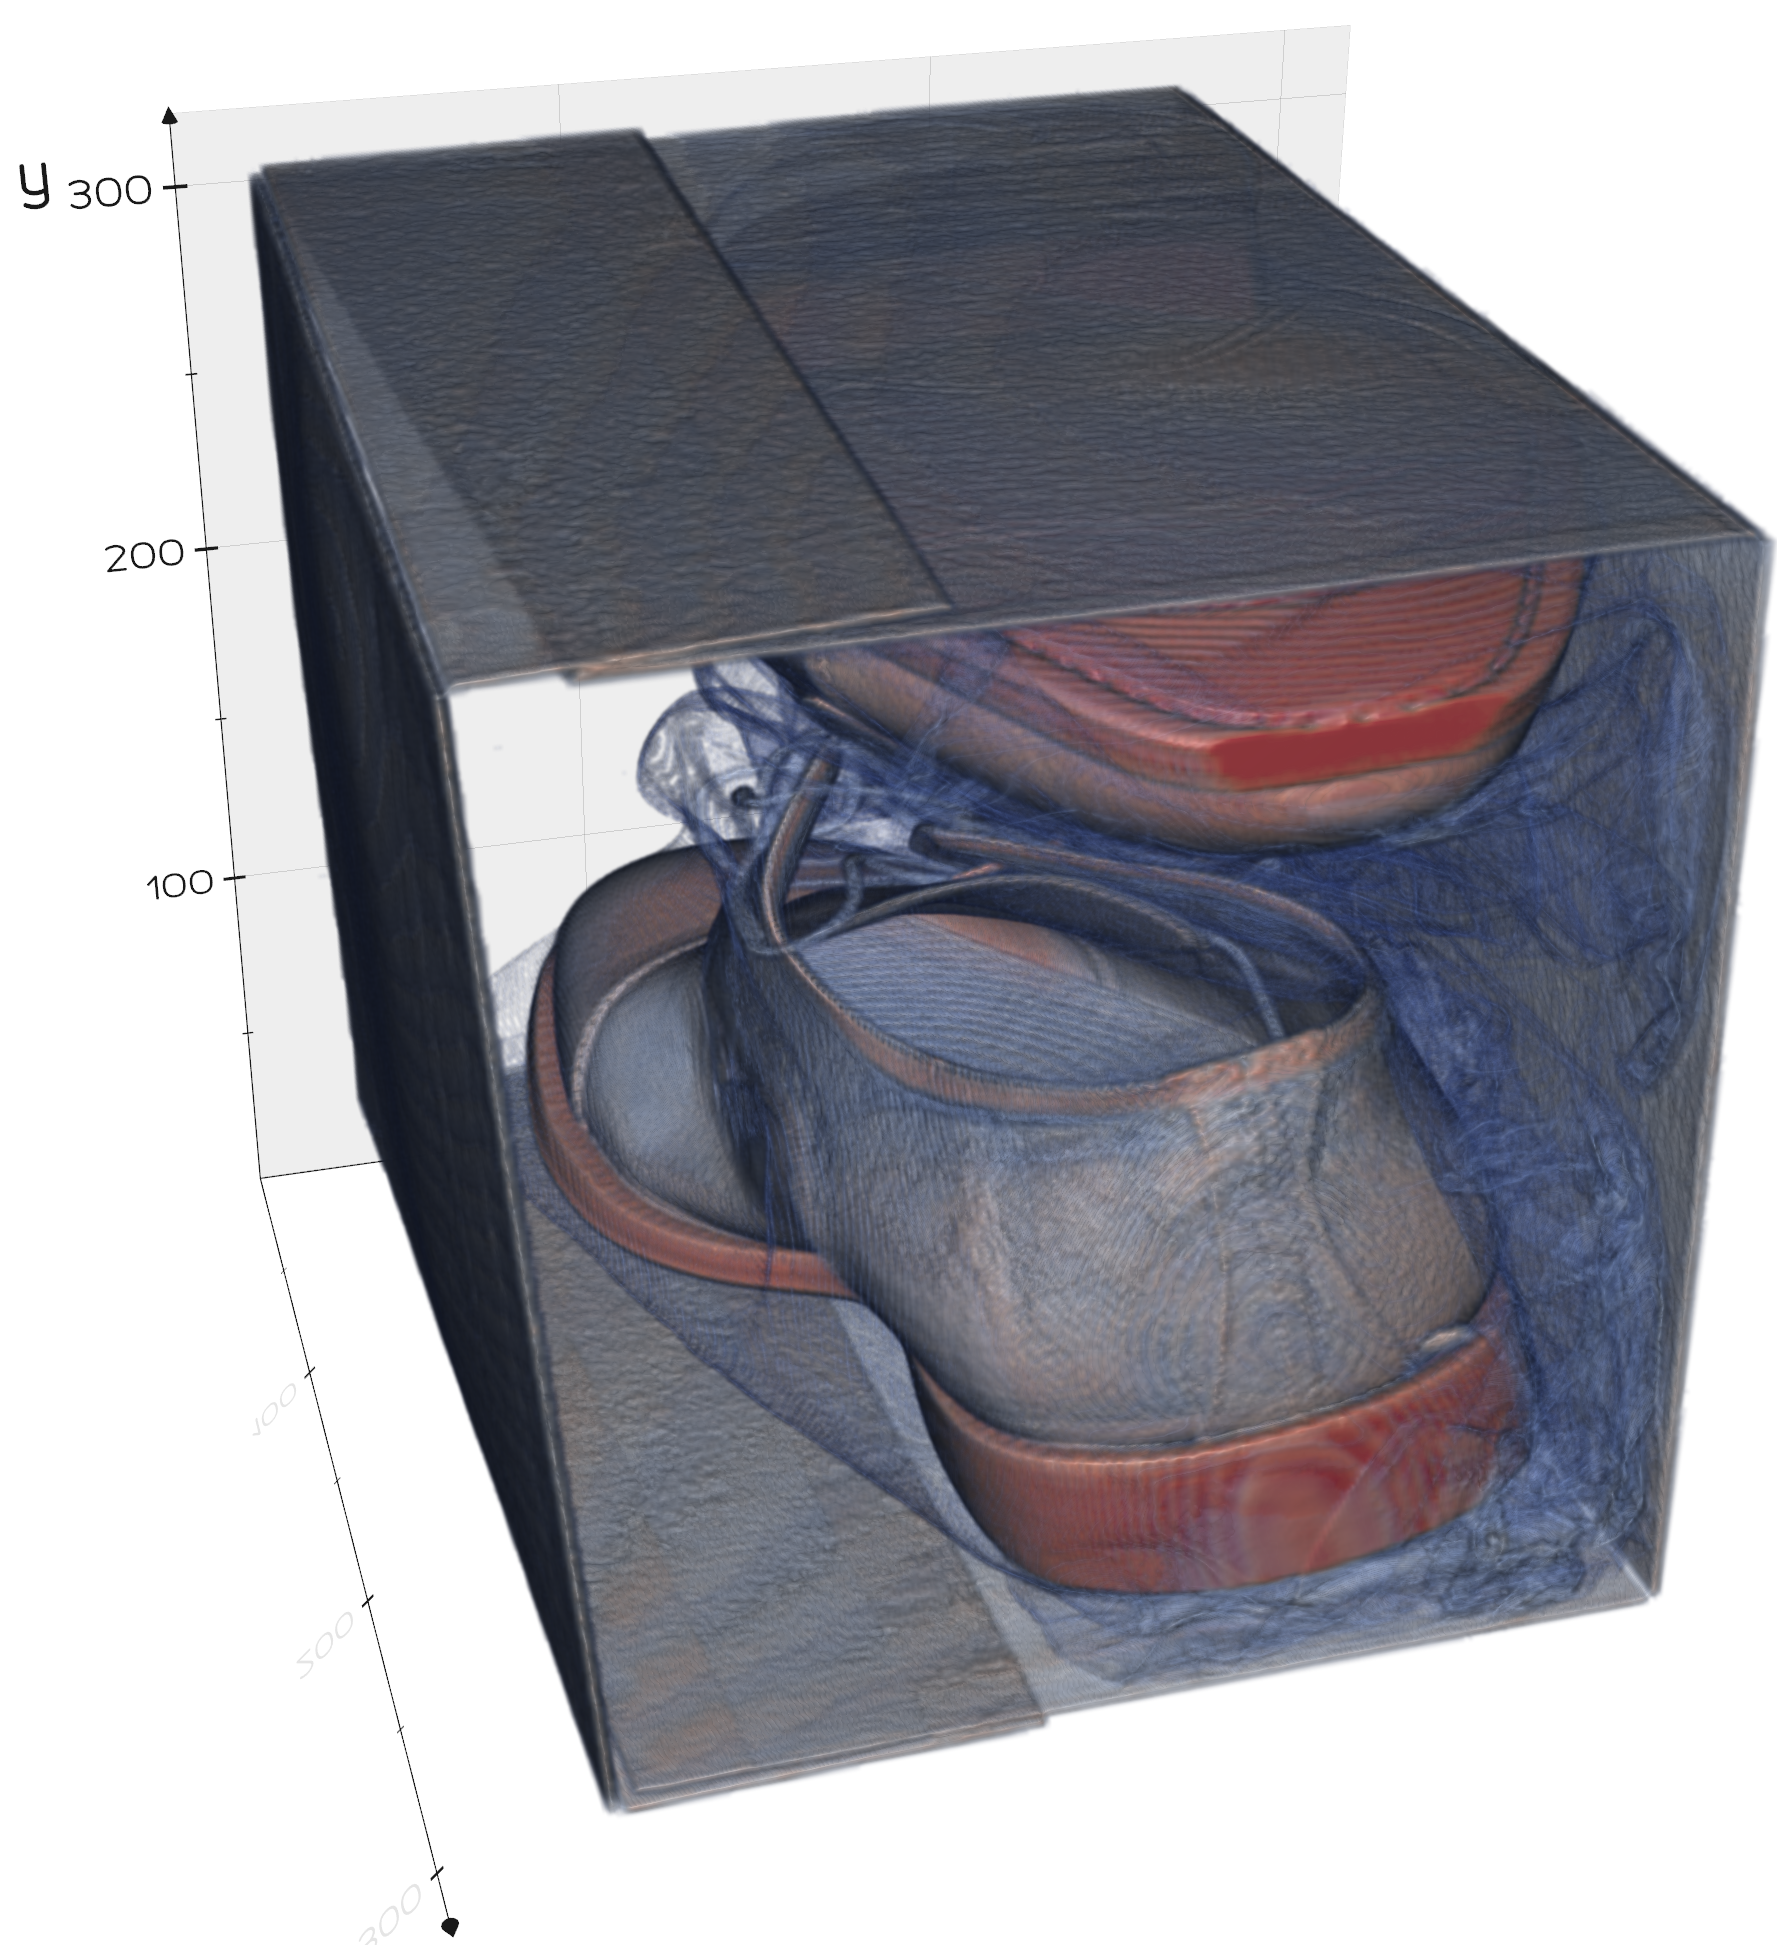
\includegraphics[width=1.0\textwidth]{./images/Bruschi_down2_2_2_3d.png}
	\end{minipage}%
	\begin{minipage}{.5\textwidth}
		\centering
		\centering
		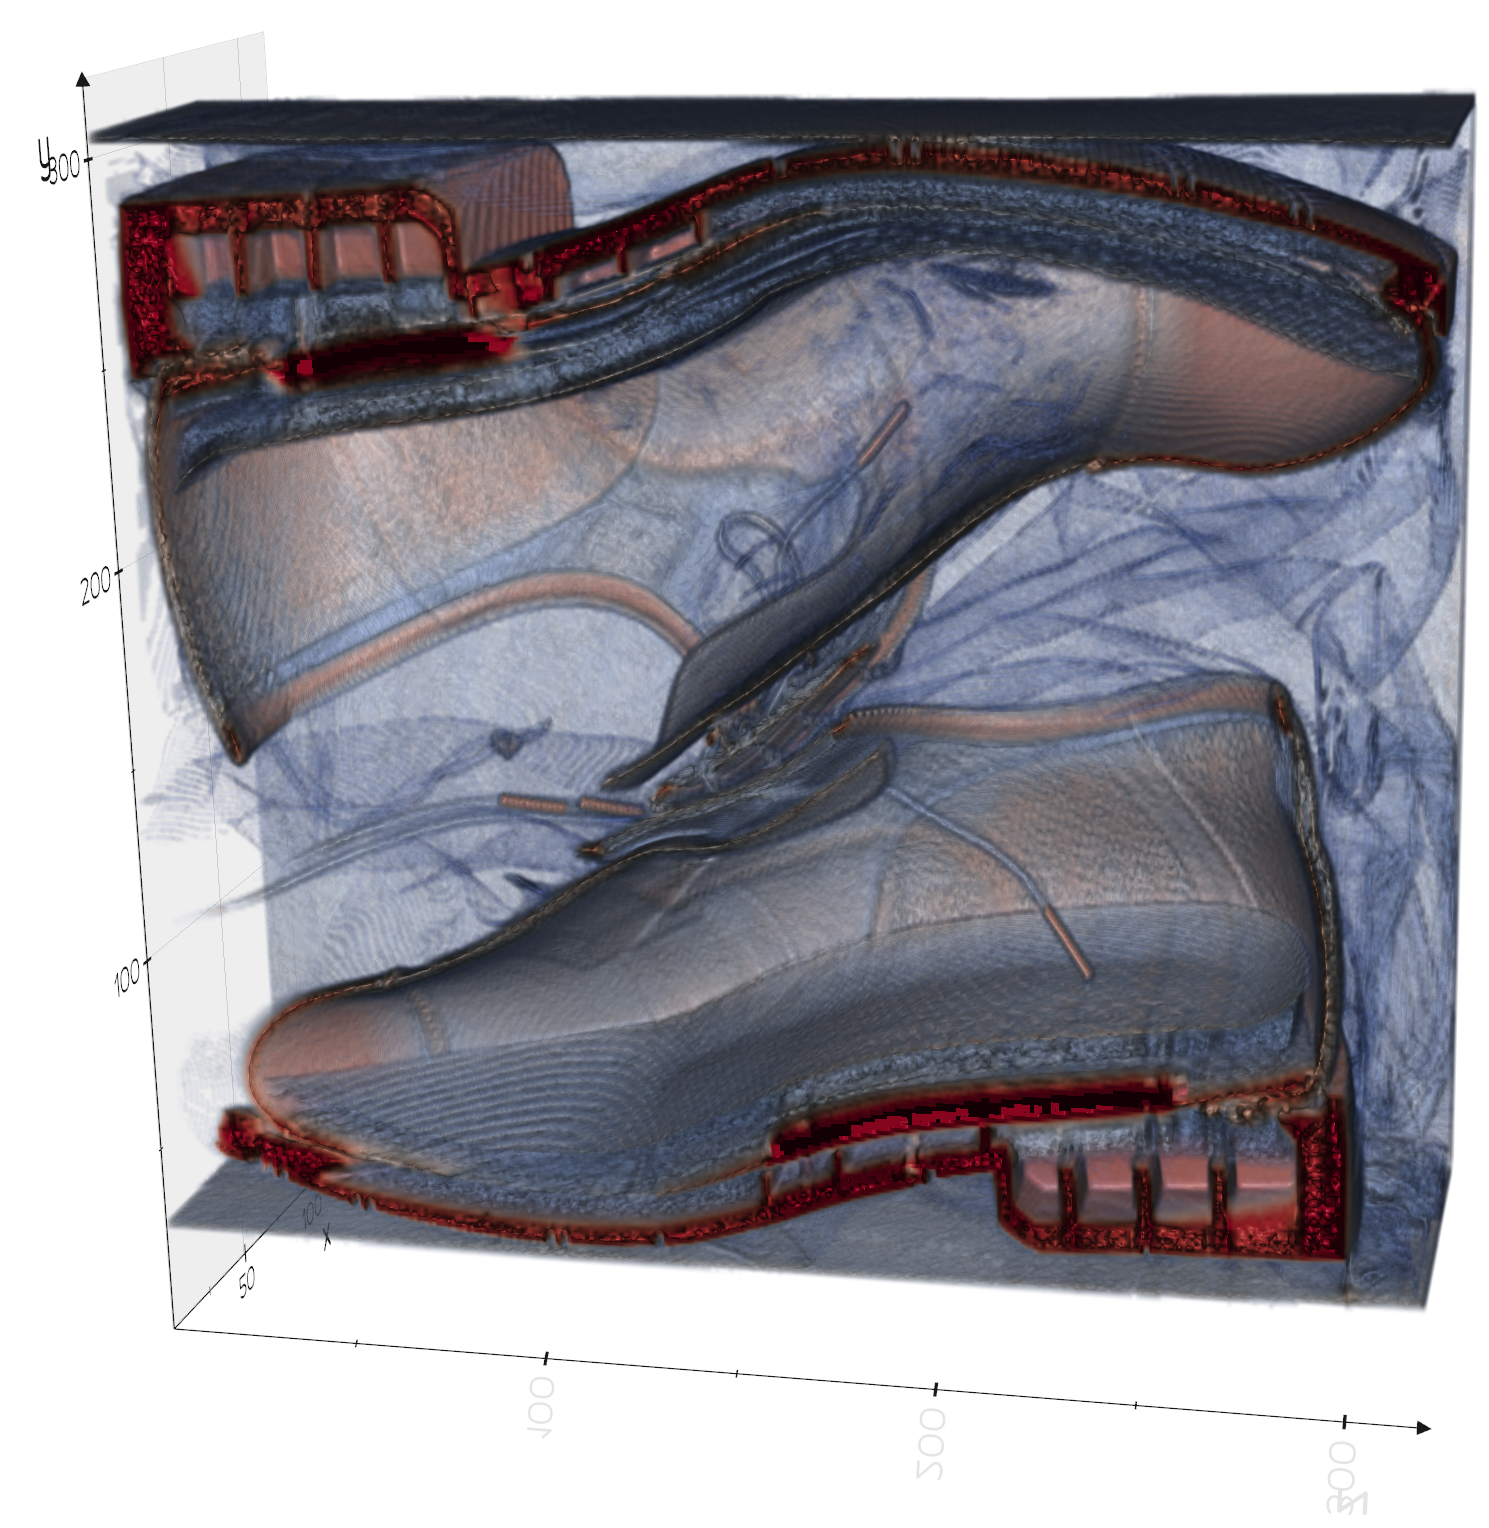
\includegraphics[width=1.0\textwidth]{./images/Bruschi_down2_2_2_3d_half.png}
	\end{minipage}
	\caption[3D-scan of {\tt Bruschi\_down2\_2\_2.rek}]{3D-scan of {\tt Bruschi\_down2\_2\_2.rek} with the original resolution of {\tt (876,650,475)} downsampled to {\tt (320,320,320)}.}
	\label{Bruschi_down2_2_2_3d}
\end{figure}

Another display variant consists of a series of slices taken from the scan. Figure \ref{Bruschi_down2_2_2} shows 24 cross-sections of the same shoe. In these images, the pair of shoes inside the box is visible and the soles, upper materials, box, and packing materials are clearly distinguishable.
\begin{figure}[H]
	\centering
	\includegraphics[width=1.0\textwidth]{./images/Bruschi_down2_2_2.png}
	\caption[File {\tt Bruschi\_down2\_2\_2.rek} with the resolution {\tt (876, 650, 475)}]{File {\tt Bruschi\_down2\_2\_2.rek} with the resolution {\tt (876, 650, 475)}. Shown are 24 different layers representing the third dimension.}
	\label{Bruschi_down2_2_2}
\end{figure}

When retrieving the associated segmentation plots for the file {\tt Bruschi\_down2\_2\_2}, the 12 segment names are {\tt Background}, {\tt Schuh\_1}, {\tt Schuh\_2}, {\tt Karton}, {\tt Innenvolumen\_1}, {\tt Innenvolumen\_2}, {\tt Ober\-material}, {\tt Innensohle}, {\tt Au(ß)ensohle}\footnote{When extracting the labels, the German umlauts and the 'ß' character are not displayed.}, {\tt F(ü)llmaterial}, {\tt Zunge}, {\tt Dummyschuh}. The label {\tt Dummyschuh} was originally introduced as a temporary helper class to combine the masks of both shoes into a single segment. However, this label was never actually used in the training or evaluation pipeline and is therefore not relevant for the segmentation task. Its presence in a few files results from it not being fully removed during preprocessing.

\medskip

Due to inconsistencies in the ordering of labels across annotation files, labels were not assigned based on index positions. Instead, each segment was identified and assigned according to its label name to ensure correctness regardless of order. This approach ensured that label mappings remained robust even when annotation files differed in structure or completeness.

\medskip

Only the six segments {\tt Karton}, {\tt Außensohle}, {\tt Innensohle}, {\tt Obermaterial}, {\tt Zunge}, and {\tt Füllmaterial} are used as ground-truth labels for the segmentation for the training of the model. The original {\tt Background} image provided in the dataset could not be used because it was incorrect. It should highlight only regions that do not belong to any of the shoe or packaging components. However, the original version contained inconsistencies; for example, some parts of the shoes were marked as background. Therefore, a new background mask was created by inverting the sum of the six segments mentioned above. The background, as shown in figure~\ref{Bruschi_down2_2_2_Segmentation}, is now correct.

\begin{figure}[H]
	\centering
	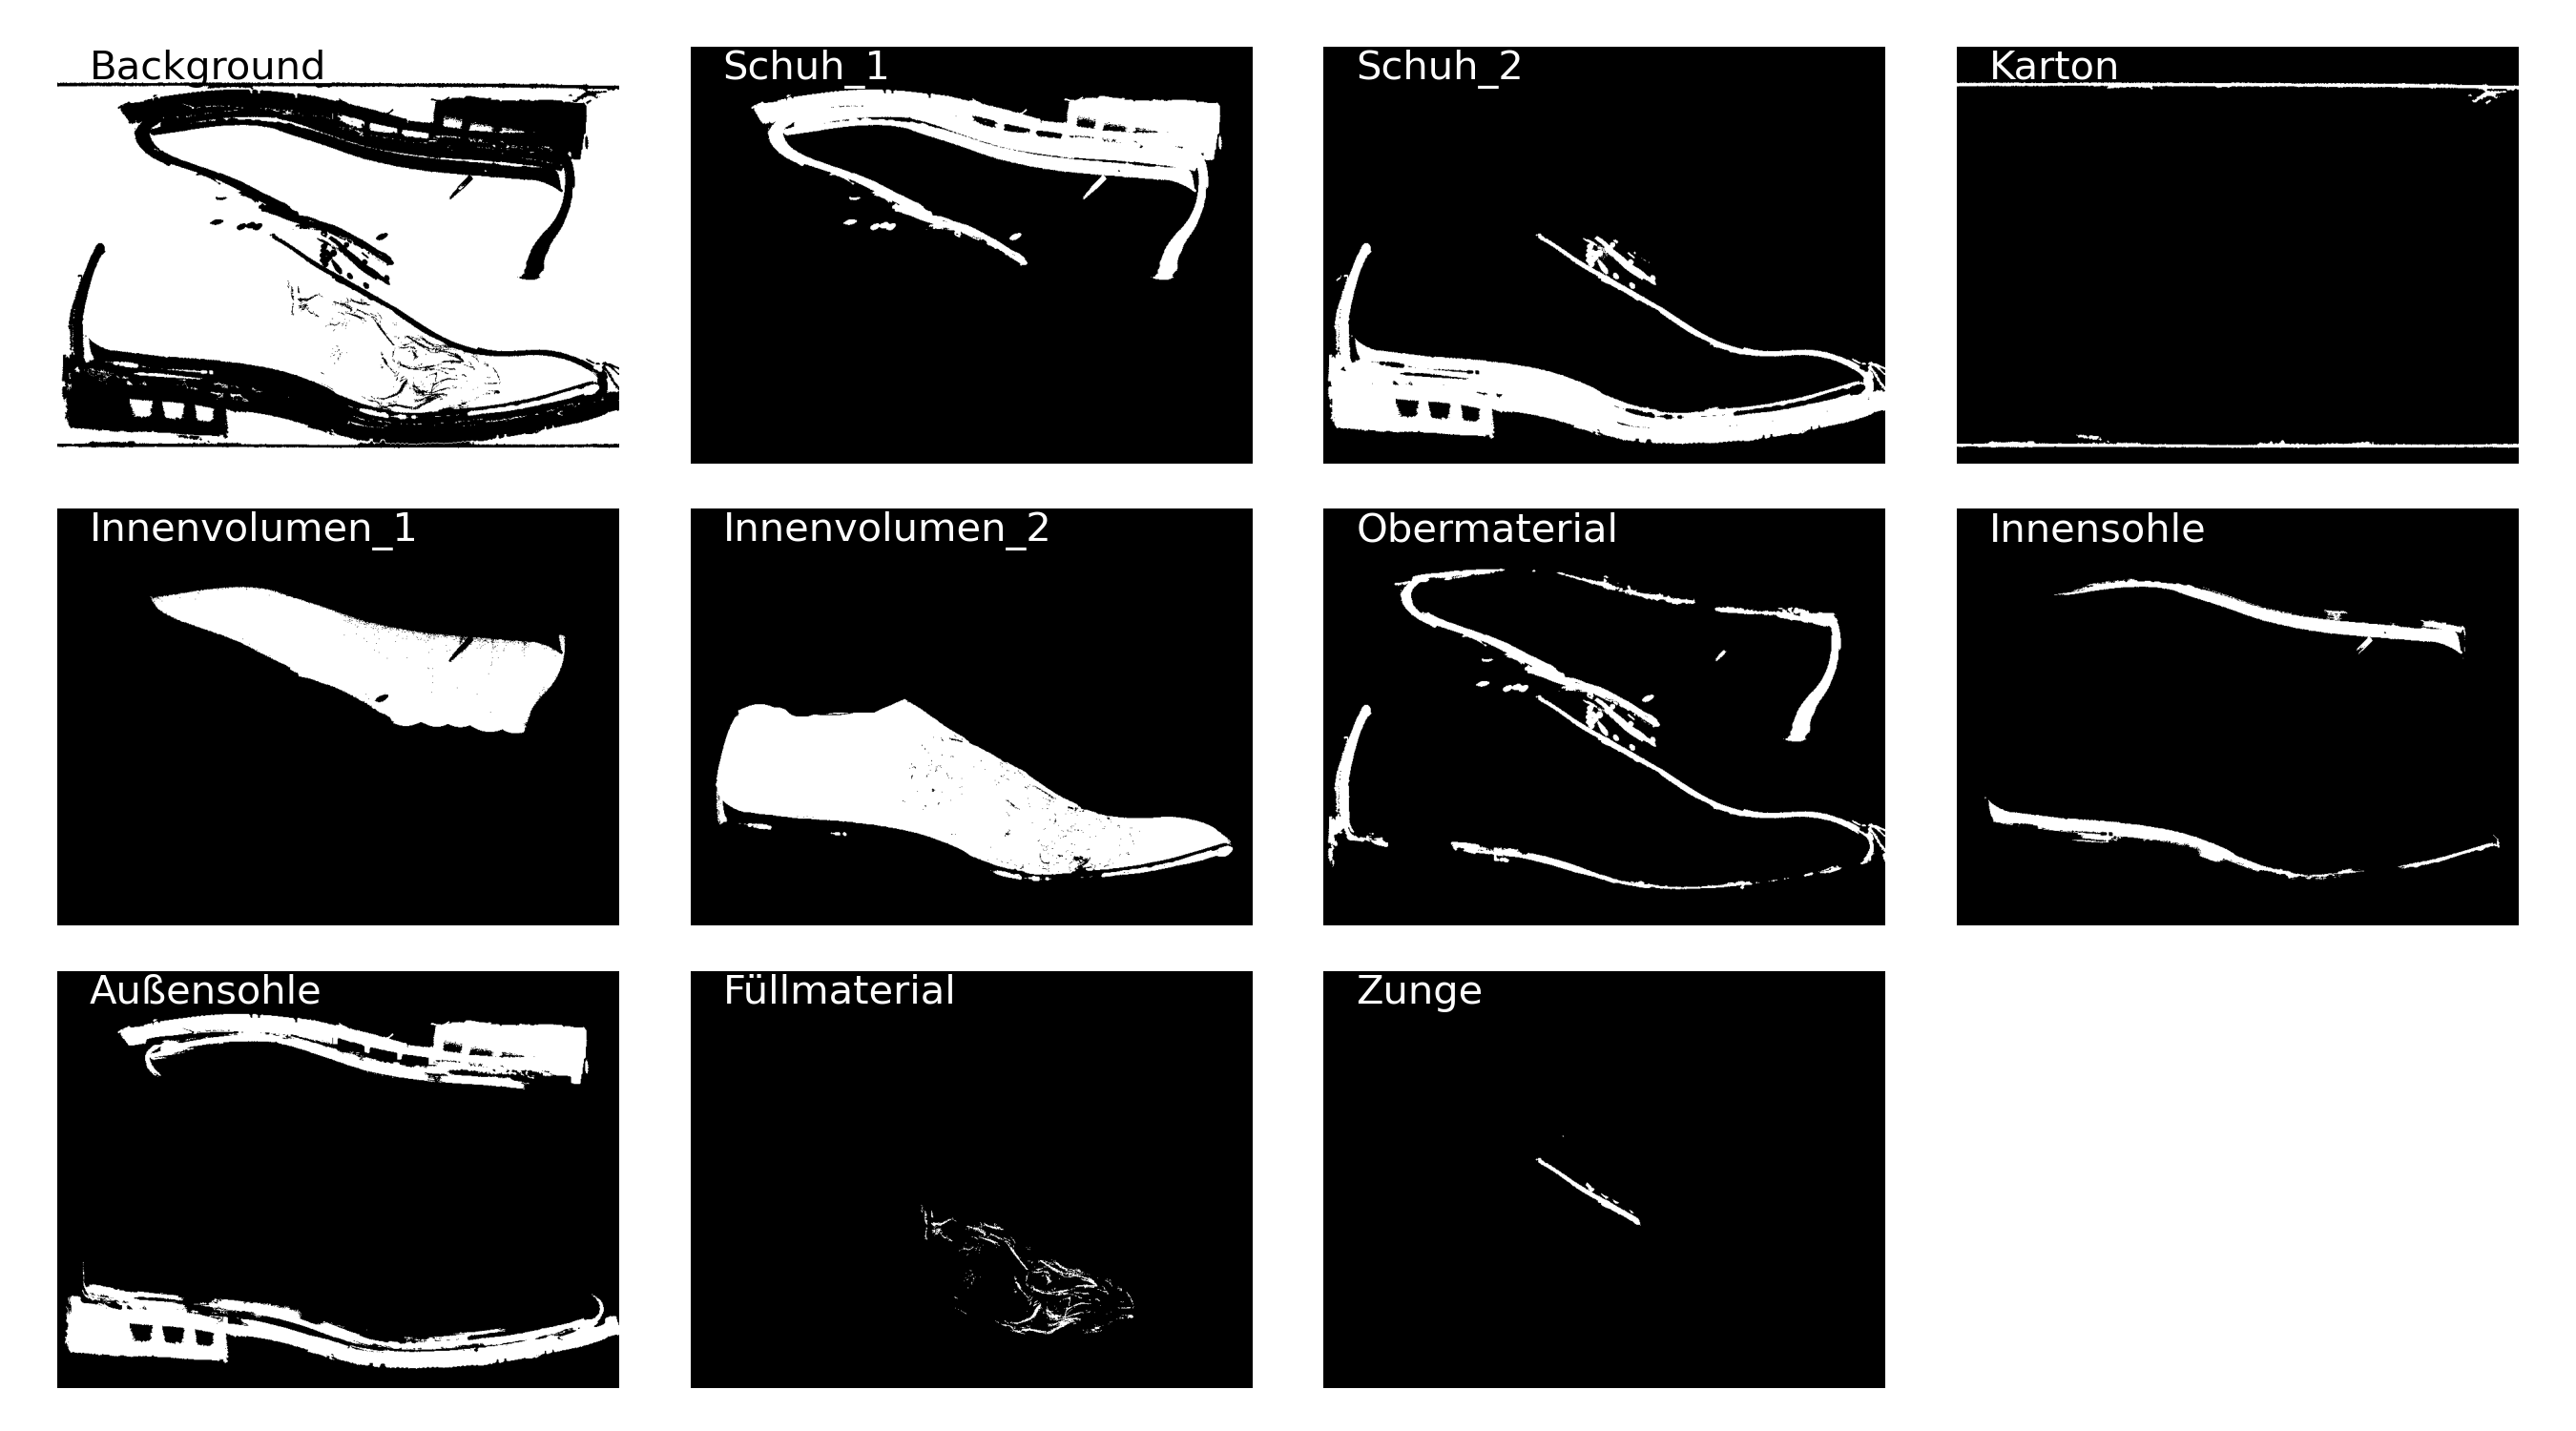
\includegraphics[width=1.0\textwidth]{./images/Layer_335_v2.png}
	\caption[Visualisation of all 11 segments for annotation file {\tt Bruschi\_down2\_2\_2}]{Visualisation of 11 segments for annotation file {\tt Bruschi\_down2\_2\_2.seg.nrrd}, Layer: 335}
	\label{Bruschi_down2_2_2_Segmentation}
\end{figure}

For the segmentation of the \gls{2d} images, a representative layer was selected by hand for each shoe somewhere in the middle of the \gls{3d} data set. The orientation for seven pair of shoe scans was also adjusted so that they can be seen in the sectional plane from the side. The shoe images were saved under the file name of the {\tt rek} file, and the seven label or segment images under the name of the annotation file. The image/segment files are assigned via key-value pairs in a dictionary. 

\medskip

The preprocessing step involves generating input volumes that are scaled to a cubic shape with dimensions depth (D) $\times$ height (H) $\times$ width (W), whereby depth, height, and width was set to be equal.  The segmentation file is then created by downscaling this volume by a factor of $2^N$ where $N$ is the number of {\tt Conv2d} or {\tt Conv3d} layers used in the overlay patch embedding module of the model head (see also figure \ref{Architecture_of_SHViT}). The downsampled segmentation volume also retains equal dimensions across all three axes. For example, if the input volume has dimensions {\tt (224, 224, 224)} and the overlay patch embedding contains two {\tt Conv3d} layers, the resulting segmentation files will have dimensions {\tt (56, 56, 56)}, due to the cumulative downscaling factor of $2^2=4$.



\section{Data Augmentation used for Training}
Data augmentation is essential when training deep learning models on small datasets. Given the limited availability of only 40 volumetric shoe scans, the network faces a significant risk of overfitting and reduced generalization \cite{HaoDataAugmentation}. Augmentation of the training set with transformed copies of each volume artificially expands the dataset and better approximates the true data distribution. Segmentation tasks in particular usually rely heavily on both the quantity and the quality of ground truth data and annotation of \gls{3d} volumes is very costly \cite{SutassananonDataAugmentation}. To avoid this, augmentation techniques that apply geometric transforms to the \gls{3d} volumes are commonly deployed. More generally, surveys of segmentation on small datasets emphasize that \enquote{data augmentation techniques are of great importance} because collecting sufficient volumetric annotations is \enquote{notoriously difficult} \cite{AlomarDataAugmentation}.

\medskip

In addition to the limited number of labeled volumes, recent studies emphasize the relationship between model complexity and required dataset size. Alwosheel et al.~\cite{ALWOSHEEL2018167} suggest that, to achieve stable generalization and avoid overfitting, the number of training samples should be at least ten times the number of trainable parameters. Given that the segmentation model used in this work contains approximately 13.8 million trainable parameters, and each \gls{3d} scan provides approximately 11.2 million voxels\footnote{Each volume has a resolution of {\tt (224,224,224)}, resulting in roughly 11.2 million voxels. If each voxel is seen as an independent training sample, at least ten volumes would be required to match the 1:10 data-to-parameter ratio for the \gls{shvit_csa} model. However, because of strong spatial correlations between neighboring voxels in semantic segmentation, the effective number of independent samples per scan is actually lower than it might appear. As a result, substantially more shoe volumes are needed, potentially 10 to 50 times more, depending on model complexity and data redundancy, as discussed in \cite{ALWOSHEEL2018167}.}, neither a single volume nor ten volumes provide a sufficient number of independent training samples. This further underlines the importance of applying targeted data augmentation to synthetically increase both the size and variability of the dataset.

\medskip

Data augmentation should be matched to the nature of the dataset, ideally reflecting its intrinsic variations. In the case of the shoe dataset, only horizontal flipping and $90^\circ$ rotations were applied, as these transformations align with the realistic orientations found in the scanned volumes. Shoes are generally placed in a consistent and orderly manner within the boxes, rather than in random or chaotic positions. Additionally, variations in brightness were observed, caused by fluctuations in exposure time that differ between individual \gls{ct} scans.

\medskip

To increase the diversity of the shoe-volume dataset, several standard volumetric augmentation methods are applied. In \gls{3d} space, simple affine transformations can generate new views of each shoe without altering its shape. In addition to geometric transformations, adjustments to brightness and contrast are also employed to simulate variations in scan conditions and improve model robustness. Commonly used operations include \cite{HaoDataAugmentation, AlomarDataAugmentation, SutassananonDataAugmentation}:
\begin{itemize}
	\item Axis-aligned flips (mirroring): Reflecting the volume across one of its principal planes (e.g. sagittal, coronal or axial) produces a mirror image of the shoe. This is equivalent to swapping one coordinate axis (for example flipping left-right across the sagittal plane). Flips preserve all voxel neighborhoods and create a valid alternative orientation. In practice, mirroring along each axis can roughly double or triple the dataset size (depending on symmetry).
	
	\item $90^\circ$ Orthogonal rotations: Rotating the entire \gls{3d} volume by $90^\circ$, $180^\circ$, or $270^\circ$ about any of the three coordinate axes creates new views. For instance, turning the shoe scan by $90^\circ$ around the vertical (z) axis creates a different front-back orientation, while a $90^\circ$ rotation about the left-right (x) axis tilts the shoe forward. By applying rotations in $90^\circ$ increments it is ensured that voxel values remain aligned on the grid (no interpolation artifacts) and the shoe's shape is preserved.
	
	\item Combined transforms: These basic flips and rotations can be composed to create additional variations. For example, a shoe volume might first be flipped left–right and then rotated $180^\circ$ about the vertical axis, resulting in a novel viewpoint. Each combination still preserves the shoe geometry while presenting it differently.
	
	\item To make the system more reliable under different \gls{ct} imaging conditions, the brightness and contrast of the voxel intensities are increased. Brightness augmentation means adding a small value to all voxel numbers to mimic changes in exposure levels. In contrast, contrast augmentation rescales voxel intensities relative to the mean, thereby enhancing or diminishing the distinction between dense and less dense regions. These transformations preserve the structural integrity and spatial relationships within the volume while enabling the network to generalize more effectively to scans acquired under different imaging settings or with varying material compositions. For the augmentation, brightness values are randomly selected from the set {\tt [-0.2, -0.1, 0.0, 0.1, 0.2]}, and contrast factors from {\tt [0.8, 0.9, 1.0, 1.1, 1.2, 1.3]}. Given the \gls{3d} volume \enquote{vol}, the following formulas are applied:
	\begin{align}
		\text{vol} &= (\text{vol} - 0.5) \cdot \text{contrast} + 0.5 \\
		\text{vol} &= \text{vol} + \text{brightness}
	\end{align}
	After applying these transformations, voxel intensities are clipped to the range {\tt [0,1]} to maintain valid intensity values.
\end{itemize}

Each of these augmentations produces a new training example. When applied to all 40 original scans, the effective training set grows by a factor equal to the number of distinct transforms used. Importantly, because these are rigid-body transformations, the ground-truth segmentation masks can be identically transformed (flipped or rotated) to match the augmented volumes. This guarantees label consistency because the shoe and its segmentations rotate together. 

\medskip

This method of increasing the size of volumetric datasets is well documented and has been proven to enhance segmentation accuracy in similar medical imaging problems \cite{HaoDataAugmentation, AlomarDataAugmentation, SutassananonDataAugmentation}. By applying these augmentations, the model can better generalize from only 40 original scans to the full variability of real-world shoe orientations and \gls{ct} imaging conditions, such as differences in brightness and contrast.

\medskip

While data augmentation is a practical and effective strategy to reduce overfitting, recent findings suggest that modern deep neural networks are capable of generalizing well even on small, noisy datasets. Olson et al.~\cite{NEURIPS2018_fface838} demonstrated that large neural networks can achieve strong performance on datasets with only a few hundred training examples, without necessarily overfitting. Their analysis shows that overparameterized networks behave like ensembles of low-bias, weakly correlated sub-networks, which introduces an implicit regularization effect. This supports the rationale for applying deep learning models even in small-data settings, especially when combined with targeted augmentation strategies that reflect the domain-specific structure of the data.

\medskip

There is no contradiction between the importance of data augmentation for small \gls{3d} segmentation datasets and the findings of Olson et al. Instead, both perspectives are complementary: data augmentation helps mitigate the high cost and limited availability of annotated volumetric data, while the study by Olson et al.~demonstrates that modern deep neural networks are capable of generalizing well, even when trained on small datasets \cite{NEURIPS2018_fface838}. This is particularly relevant when combined with suitable augmentation strategies. Together, these approaches enable effective training of deep models in scenarios where large-scale labeled data is not available.


\section{Implementation Details}
Before training, all input data undergo a structured preprocessing pipeline to ensure consistency and compatibility with the segmentation model. The preprocessing procedure consists of two main stages: processing the volumetric image data and preparing the corresponding annotation files.

\medskip

In the first stage, each shoe scan, which is stored as a \gls{3d} volume, is loaded from disk. To establish a uniform viewpoint across the dataset, some of the volumes are rotated such that all shoes are viewed consistently from the side. Following this orientation correction, all volumes are resized to a common cubic shape, meaning that the height, width, and depth of each volume are scaled to the same fixed value. This same resizing guarantees that all inputs have identical dimensions, which is particularly important when working with \gls{3d} convolutional neural networks, as it simplifies the design of the model and ensures spatial uniformity. After resizing, brightness normalization is applied as described in section \ref{sec::visualizing_the_volumes}, where pixel intensity values are scaled and clipped based on fixed percentile thresholds. The preprocessed volumes are then saved in NumPy format for downstream processing with only one \enquote{color} channel.

\medskip

In the second stage, the corresponding annotation files are handled. Each annotation file contains a full voxel-wise segmentation map in which multiple segments or labels are defined (see also section \ref{sec::visualizing_the_volumes}). For the purposes of this work, only seven (including background) specific labels are retained. These selected segments represent the most structurally and semantically relevant parts of the shoe. The segmentation volumes are then rotated using the same transformation applied to the associated shoe volume to preserve alignment. Next, the label volumes are resized according to the spatial resolution required by the segmentation head of the network, taking into account the number of convolutional layers and their respective downsampling effects.

\medskip

Finally, the segmentation labels are stored in a single \gls{3d} NumPy array per shoe, where voxel values range from 0 (background) to 6, with each integer value uniquely representing one of the seven selected shoe segments. This compact and standardized format ensures efficient loading during training and allows for direct compatibility with loss functions that expect integer-coded segmentation masks.

\bigskip

This study implemented the standard SegFormer with \gls{mvt} and \gls{shvit} backbones using PyTorch. TensorFlow was initially considered for the implementation. However, a memory leak was observed during its use, with the available \gls{gpu} memory gradually decreasing over time. This issue has been documented in TensorFlow's GitHub issues and has persisted without resolution\footnote{\url{https://github.com/tensorflow/tensorflow/issues/61791}}. Notably, it is present since TensorFlow v2.11 but was not seen in v2.9. To mitigate this issue, the TensorFlow code of SegFormer was ported to PyTorch, which offers more transparent memory management and enhanced control over resource allocation.
\gls{shvit} was already coded in PyTorch, thus requiring only minor adjustments to harmonize the interfaces for \gls{mvt} and \gls{shvit}.

\medskip

Furthermore, the code initially developed for \gls{2d} applications was restructured to also process \gls{3d} volumetric scans. A notable enhancement was the integration of the sliding-window attention mechanism, elaborated upon in the preceding section (see section \ref{Transformer_Attention_Mechanisms}). The original source code, taken from the \gls{simvit} GitHub repository\footnote{\url{https://github.com/ucasligang/SimViT/blob/main/classification/simvit.py}}, underwent slight modifications. Notably, the Python scripts are designed to function without installing additional libraries, such as {\tt timm}\footnote{\url{https://pypi.org/project/timm/}}, which is often used.

\medskip

To allow experiments with \gls{shvit} focusing on variables such as kernel size and the use or omission of central self-attention, additional modifications were made to the initialization routines of the respective classes. Details of the entire code are available in appendix \ref{sec::shvid_3d.py}, on pages \pageref{sec::shvid_3d.py}ff.

\medskip

The {\tt \_\_init\_\_} functions of the two SegFormer models, {\tt SegFormer3D} (with \gls{mvt}) and {\tt SegFormer3D\_SHViT}, were designed to accept the same input parameters, even if some were not used universally. This approach allows the models to be easily interchanged without requiring modifications to the model invocation in the main program.

\medskip

The main program used for training is a Jupyter notebook file. In this file, the model is loaded, and the data loaders are initialized for training, validation, and test datasets with augmentation. Additionally, the functions for the F1-score metric and -loss are defined. The program includes callbacks for warm-up, early-stopping, logging, and saving model parameters if improvements in the validation metrics occur.

\medskip

The training function begins with a warm-up phase reserved for the initial 20 epochs, during which the learning rate gradually increases to its target value. Following the warm-up, the actual training process starts, utilizing gradient accumulation with  {\tt BATCH\_SIZE=1} and {\tt ACCUMULATION\_STEPS=5}. After the data loader is applied to the training data, validation is conducted using the validation dataset to evaluate F1-score and -loss.

\medskip

Although data augmentation techniques are used to artificially expand the dataset, the underlying diversity remains limited to the original 40 shoe-samples. Cross-validation ensures that the models's ability to generalize is tested across different subsets of the original base shoes because normal train-test-splits can result in insufficient data for either training or validation purposes. Cross-validation, with {\tt kFold=5} in this thesis, addresses this limitation by utilizing every sample for both training and validation across different folds, thereby maximizing the informational value extracted from available data. It is important that the same original image does not appear in both training and validation sets within the same fold \cite{Kohavi_1995, Arlot_Celisse_2010}. Known as \enquote{data leakage prevention}, this principle maintains the independence between training and test data, and it is fundamental to get unbiased performance estimates\footnote{see also section 2.4 of \cite{Kapoor_Narayanan_2023}}. 

\medskip

At the end of each epoch, the F1-score and -loss values for both training and validation are displayed. If no improvement in validation F1 is observed within a specified number of epochs, the learning rate is reduced and the internal counter is reset, and training continues. Should the metric still fail to improve within another set of epochs, early stopping is triggered and training is terminated.

\medskip

Finally, curves for F1-score and -losses during training and validation are plotted. The best model, determined by the lowest validation loss, is loaded and used with the test dataset. All input images or volumes are loaded, segmentation predictions are generated, and the results are visualized by comparing the original input, the predicted segmentation, and the ground truth.
